This section talks about the layer of the robot arm and how each components are going to interact with necessary data inputs to perform the task of palletizing and depalletizing the boxes. The primary goal of this layer is to interact with the boxes and configure the necessary position the arm needs to be in to execute the task.
\begin{figure}[h!]
	\centering
 	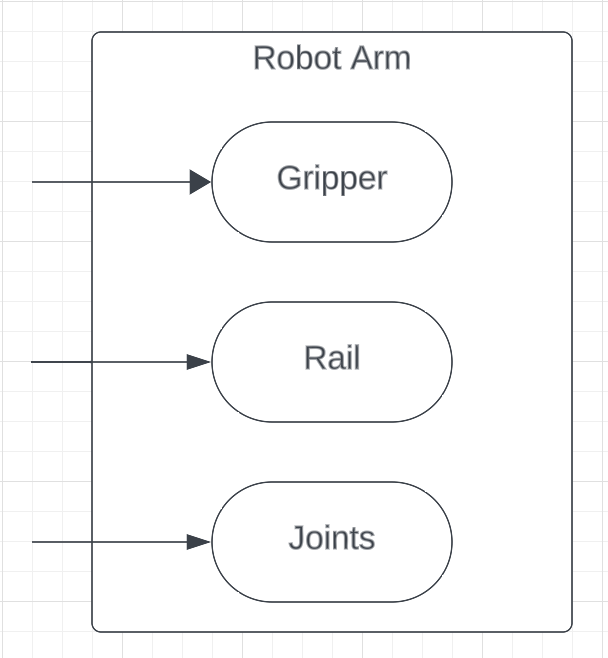
\includegraphics[width=0.60\textwidth]{images/arm}
 \caption{Robot Arm diagram}
\end{figure}


\subsection{Gripper}
This layer consists of the gripper which primarily requires the use of the hydraulic suction to create or remove grip to the boxes.

\begin{figure}[h!]
	\centering
 	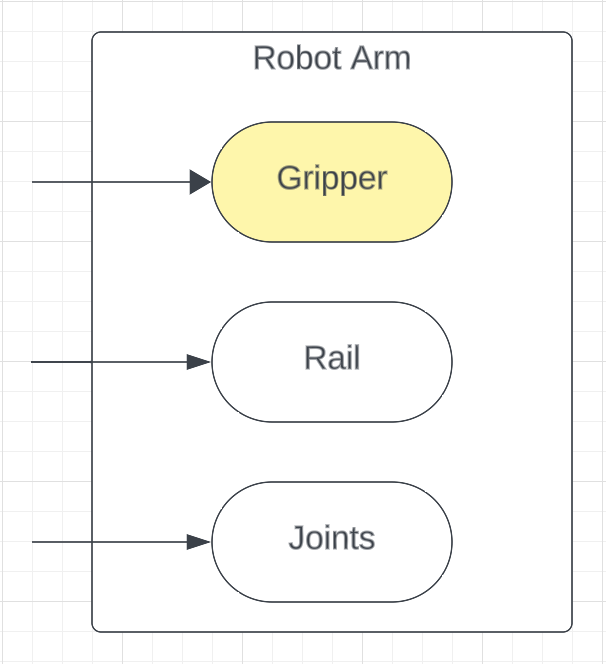
\includegraphics[width=0.60\textwidth]{images/gripper.png}
 \caption{Robot Arm diagram}
\end{figure}

\subsubsection{Assumptions}
Any wiring required for the gripper is already provided and will be stable to perform the necessary actions for the gripper to execute its task.

\subsubsection{Responsibilities}
The gripper is responsible for creating grip on to the boxes and remove any grip on to the boxes. The data to create/remove the grip comes from PLC which uses QR code to send the data to hold a grip on to the boxes and once the task is executed, the gripper is given the data to remove the hold on the boxes.

\subsubsection{Subsystem Interfaces}
\begin {table}[H]
\caption {Subsystem interfaces}
\begin{center}
    \begin{tabular}{ | p{1cm} | p{6cm} | p{3cm} | p{3cm} |}
    \hline
    ID & Description & Inputs & Outputs \\ \hline
    \#1 & Suction grip & \pbox{3cm}{Box detection} & \pbox{3cm}{hydraulic grip}  \\ \hline
    \end{tabular}
\end{center}
\end{table}

\subsection{Rail}
This layer consists of the linear rail required to give the robot arm a linear motion.

\begin{figure}[h!]
	\centering
 	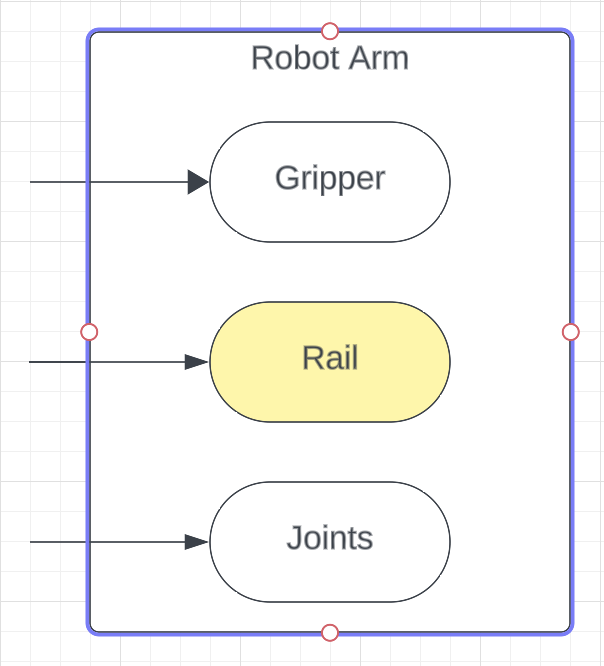
\includegraphics[width=0.60\textwidth]{images/rail.png}
 \caption{Robot Arm diagram}
\end{figure}

\subsubsection{Assumptions}
Any wiring required for the motion of linear rail is already provided and is stable when the robot arm is in motion.

\subsubsection{Responsibilities}
The linear rail is responsible for moving the entire robot arm in a linear motion in defined boundaries in order to get to a configuration to move the boxes. The linear rail will get the data from the servo amplifier which is a component of the PLC.

\subsubsection{Subsystem Interfaces}
\begin {table}[H]
\caption {Subsystem interfaces}
\begin{center}
    \begin{tabular}{ | p{1cm} | p{6cm} | p{3cm} | p{3cm} |}
    \hline
    ID & Description & Inputs & Outputs \\ \hline
    \#2 & Rail Motion & \pbox{3cm}{PLC data } & \pbox{3cm}{linear movement}  \\ \hline
    \end{tabular}
\end{center}
\end{table}


\subsection{Joints}
This layer consists of the configurations required for the arm to be able to reach the boxes.

\begin{figure}[h!]
	\centering
 	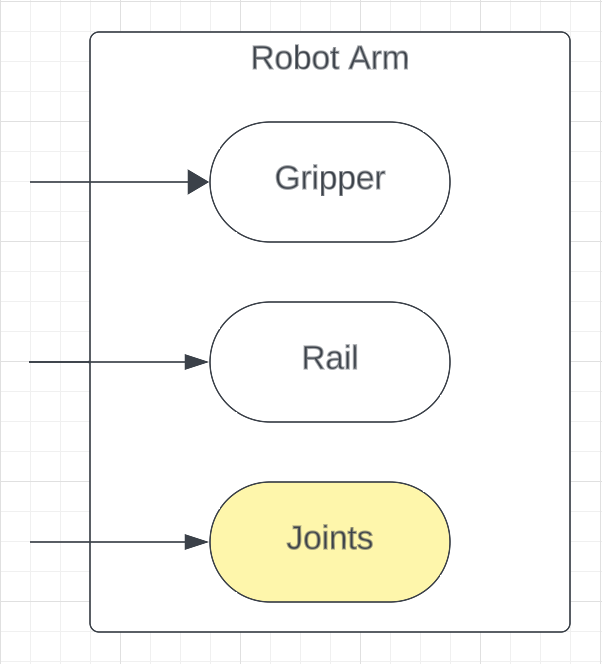
\includegraphics[width=0.60\textwidth]{images/joints.png}
 \caption{Robot Arm diagram}
\end{figure}

\subsubsection{Assumptions}
Any wiring required for the arm to be in multiple configurations is provided and would be stable while the arm is in motion.

\subsubsection{Responsibilities}
The joints are responsible for the movement of the gripper and be in a certain configuration so that the gripper is able to reach the boxes. Joints communicate directly with the PLC which gives the appropriate data to be in a certain configuration space.

\subsubsection{Subsystem Interfaces}
\begin {table}[H]
\caption {Subsystem interfaces}
\begin{center}
    \begin{tabular}{ | p{1cm} | p{6cm} | p{3cm} | p{3cm} |}
    \hline
    ID & Description & Inputs & Outputs \\ \hline
    \#2 & Joint Configuration & \pbox{3cm}{PLC data} & \pbox{3cm}{joint angle}  \\ \hline
    \end{tabular}
\end{center}
\end{table}
